\section{引言}

“世界模型”一词在不同语境中积累了多种用法，既揭示了一些含义，也掩盖了另一些含义。早在1943年，\cite{craik1943nature}便提出，生物体通过在头脑中维持物理世界的“工作模型”（working model）来生存和繁衍。这些模型使心智能够模拟假想情境、预测候选行动的结果，并预先计算最优策略，而不必完全依赖缓慢的物理试错交互。这一思想的算法实现，正是今天所谓“世界行动模型”（World Action Model，WAM）的形式化体现。Craik的假说为强化学习智能体和生成模型等重要人工智能架构奠定了思想基础\citep{sutton2018rl}。计算机视觉、机器人学和生成建模等领域都使用这一概念，但它们所指的系统往往大不相同。近年来，最有影响的概念澄清尝试是李飞飞（Fei-Fei Li）提出的功能分类：将世界模型划分为\textit{渲染器（renderer）}（生成像素）、\textit{模拟器（simulator）}（预测状态转移）和\textit{规划器（planner）}（提出行动）三类\citep{worldlabs2026taxonomy}。

这一功能分类有助于澄清概念，但它的根本局限在于：所划分的是表征（representation）的\textit{解码方式（decoding）}（也称投影），而非表征本身。一个统一的内部模型可以根据调用的查询接口，解码为RGB像素、状态向量或候选行动方案。该分类规定了世界模型输出什么，却没有定义内部模型是什么、应当如何构建。上游问题——如何构建一种共享的内部表征，以支持这三种解码——仍是功能分类尚未回答的问题。

另一种观点以\cite{lecun2022path}的论述最具代表性，认为生成式重建从来都不是正确的目标：在潜在空间（latent space）中进行预测的联合嵌入架构（joint-embedding architecture）已经足够，而像素级重建会将表征容量浪费在无关的光度细节上。我们赞同，精确的像素级重建不应成为世界模型的终极目标；不过，重建质量有助于查明压缩表征没有保留哪些信息。最终，重建对世界建模究竟有多重要，只能通过测试来判断。

关于压缩表征，如今人们普遍认为，大语言模型（large language model，LLM）擅长压缩人类的\textit{语言}知识。类似地，世界模型是一种统一的压缩机制（compression mechanism），其核心目标是尽可能压缩\textit{现实世界物理感官观测与智能体行动的联合分布}。有损压缩带来了不可避免的表征取舍，形成一条连续谱：潜在表征可以偏向紧凑的高层语义抽象，也可以优先保留细粒度物理动力学和感知保真度；所有实际世界模型都在这两个极端之间取得某种平衡。这种以压缩为中心的观点，或许更能刻画当前研究中的架构选择、数据约束和经验瓶颈。

\paragraph{数据决定能力上限}
我们的出发点是一个简单却影响深远的前提：任何智能系统在物理世界中的泛化能力上限，都由训练数据所包含的物理经验多样性决定。在架构和计算预算固定的条件下，决定这一上限的是数据多样性，而非模型结构或训练超参数。架构与计算量影响系统接近上限的效率，却不能抬高上限\citep{hoffmann2022training}。

目前，唯一能够扩展到所需多样性的物理数据来源，是开放互联网中数以千亿计的图像、视频和文本样本。专有数据来源——灵巧操作数据集、第一人称具身记录以及安装在外骨骼上的传感器——在多样性和规模上都受到结构性限制。在可预见的未来，无论部署多少硬件，都无法产生互联网规模的操作数据。因此，要构建能够泛化到物理世界的“世界模型”，就必须从现有数据中尽可能多地提取物理理解。

尤其是互联网视频，它是规模空前的自然语料库，以完全隐含的方式编码了极其广泛、具有结构的物理世界知识。日常视频的原始像素流中，蕴藏着支配物理现实的基本先验：物体恒存性（object permanence，即物体在视野之外仍持续存在）、区分刚体与可变形材料的刚性和非刚性约束、物体运动与交互的运动学限制、光照和阴影的时间变化、遮挡与显露的因果逻辑、事件的层级因果链，以及类人行动与交互的结构先验。\textit{关键困难在于，所有这些物理结构在原始像素空间中都处于潜在状态，无法直接获取。}

图\ref{fig:data1}给出了我们提出的\textbf{倒金字塔工作流（Inverted Pyramid Workflow）}，用以解决上述核心困难。原始互联网视频中蕴藏着潜在物理先验，但这些先验埋藏在无标签像素中；专有机器人硬件又无法独立产生规模和多样性相当的数据。该流程以互联网中范围极广的真实物理场景影像为基础，首先通过自动筛选和标注，释放其中潜在、隐含的物理知识，以数据多样性提高世界模型的泛化上限。随后逐级收窄的数据漏斗起到精细蒸馏的作用：去除无关视觉内容，合成标准化行动表征，只保留机器人所需、具有物理意义的运动与交互信号。最终形成规模紧凑、符合任务要求的真实世界数据集，使模型能够在具身操作任务上高效收敛，同时保留从数十亿互联网视频中提取的广泛物理先验。架构与计算量只决定模型学习的速度；这一倒置流程则扩展了训练语料中基础物理经验的多样性，提高了世界模型对未见现实物体、运动和因果情境的泛化上限，而这些内容无法被规模有限的专有机器人数据集充分涵盖。

\begin{figure}[h]
    \centering
    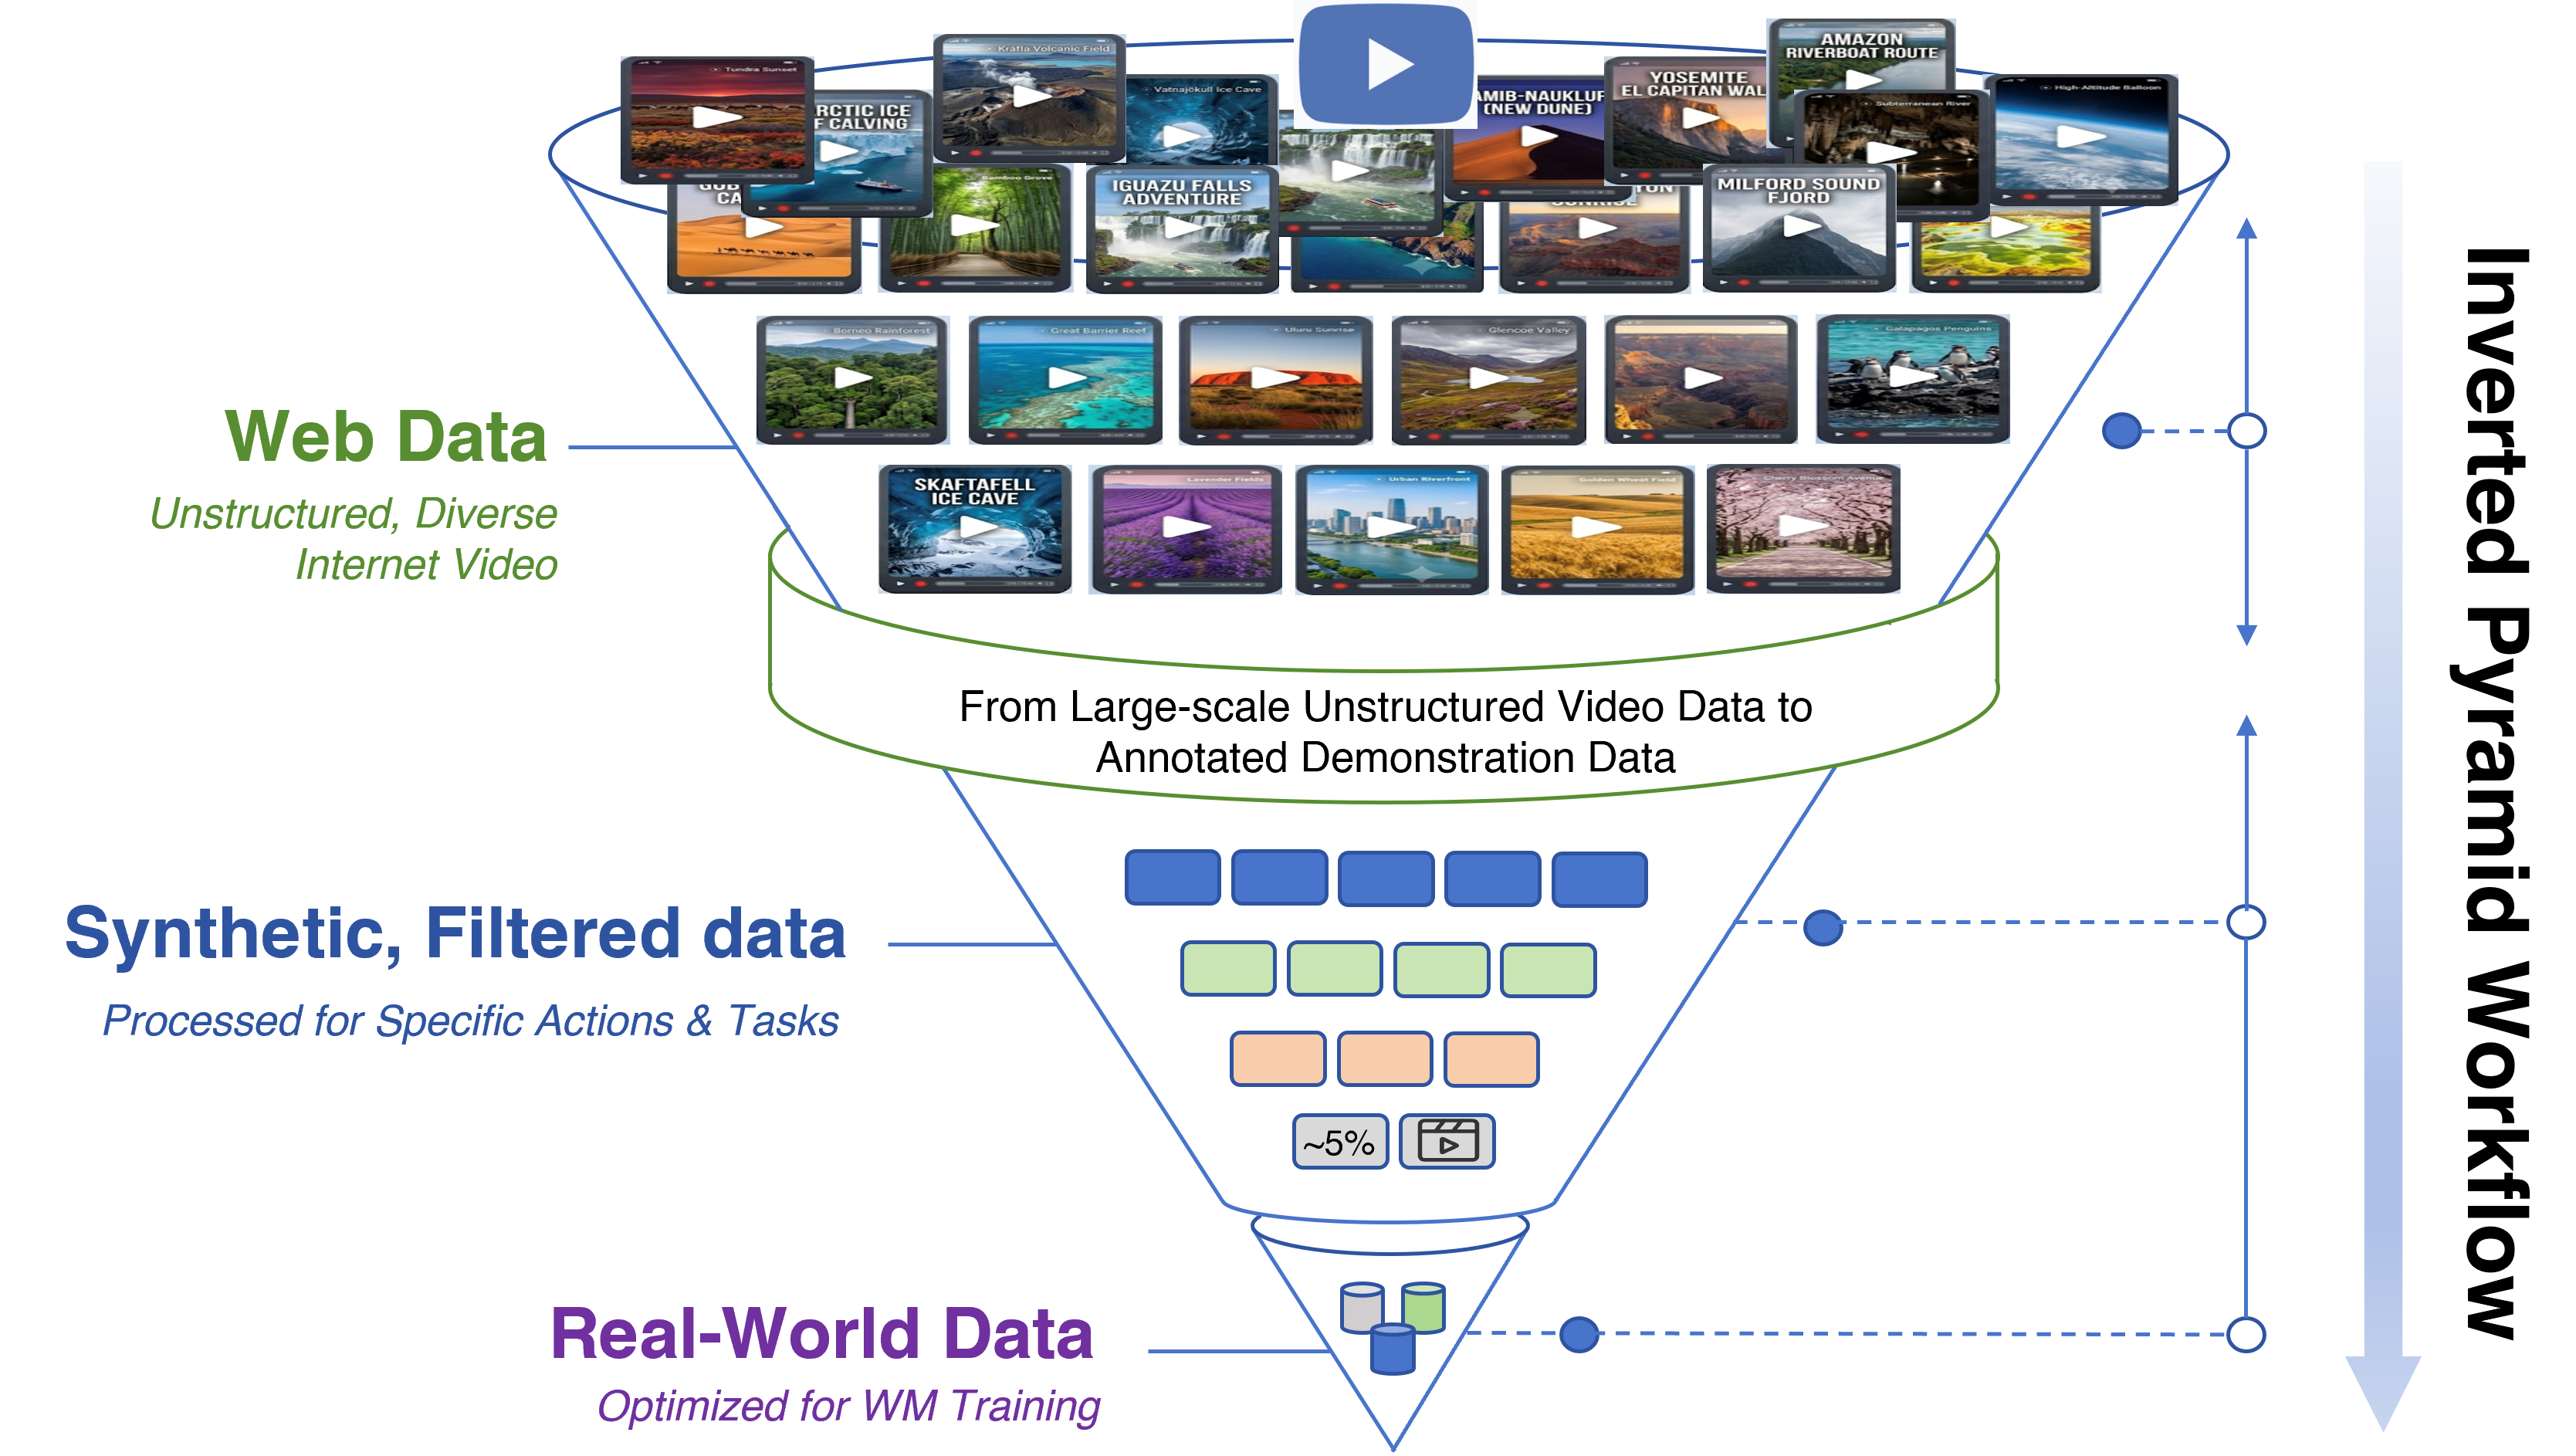
\includegraphics[width=0.85\linewidth]{figs/data4.png}
    \caption{用于机器人与物理世界模型训练的数据金字塔倒置漏斗：从海量无结构公共媒体，逐级提炼出规模紧凑、面向任务优化的机器人训练数据。最宽的顶层是“互联网数据来源”：无结构、多样化的公共视频，即数十亿段记录人类物理交互的原始像素流。中间层为“合成与筛选数据集”：经过大幅精简、为特定机器人行动与操作任务筛选及合成的数据子集。最窄的底端是“真实世界任务数据”：规模小、经过精心整理、为端到端机器人训练充分优化的数据集，其紧凑规模便于高效微调具身模型。}
    \label{fig:data1}
\end{figure}

\paragraph{作为压缩机制的世界模型}
高维视频观测主要由与任务无关的光度变化占据：视角、光照、纹理、传感器噪声和杂乱背景的变化，掩盖了底层物理规律。原始像素并不显式表征恒存性、因果性或约束，只编码表面外观，而不编码产生视觉信号的物理生成结构。因此，提取这些隐含物理先验需要一种专门设计的\textit{压缩机制}，将高维、含噪视频观测提炼为紧凑、有力且具有语义结构的表征。这种压缩的核心功能不仅是降维，而是有针对性地保留信息：准确保留下游物理推理与控制所需的结构化因果和物理信息，同时系统地舍弃原始像素数据中占主导地位、却与任务无关的光度变化。\textit{我们认为，这正是世界模型具有定义性、奠基性的任务；从根本上说，它严格属于压缩问题，而非生成或模拟问题。}生成和模拟是良好压缩表征所带来的下游能力，并非目标本身；世界模型的核心目标，是解决一个信息论问题：将高维感官数据中隐含的物理知识提炼为可用、紧凑的形式。
